\subsection{Bernoulli generalized linear model does not fully capture psychometric curves}
\label{sec:glmhmm:2.2.6}

Our inactivation experiments suggest that DMS pathways make strong contributions to behavior during a cognitively demanding evidence accumulation task, but do not contribute strongly to similar tasks with weaker cognitive demands. However, even during the evidence accumulation task, it is possible that the animals’ level of cognitive engagement varies over time. This raises the possibility that the contributions of the two pathways to behavior could change over time, even within the same task.

To address this possibility, we sought to understand the factors that contribute to decisions in the evidence accumulation task. As a first step, we used a Bernoulli generalized linear model (GLM) to predict choice based on a set of external covariates (Fig. \ref{fig:glmhmm:4}a,b). These covariates included the sensory evidence (difference between the number of right and left cues, or ‘$\Delta$ cues’), the recent choice and reward history, the delivery of optical inhibition (‘laser’), as well as a bias. Note that we set the value of the laser covariate to $+1$ (or $-1$) on trials with right (or left) hemisphere inhibition, and zero otherwise. A positive (or negative) GLM weight on this covariate thus captured an ipsilateral (or contralateral) ‘laser’-induced bias in choices relative to the hemisphere of inhibition. For the choice history covariates, a positive weight indicates a tendency toward repeating past choices (\ref{sec:appendix1:methods}).

\begin{figure}[t!]
  \begin{center}
    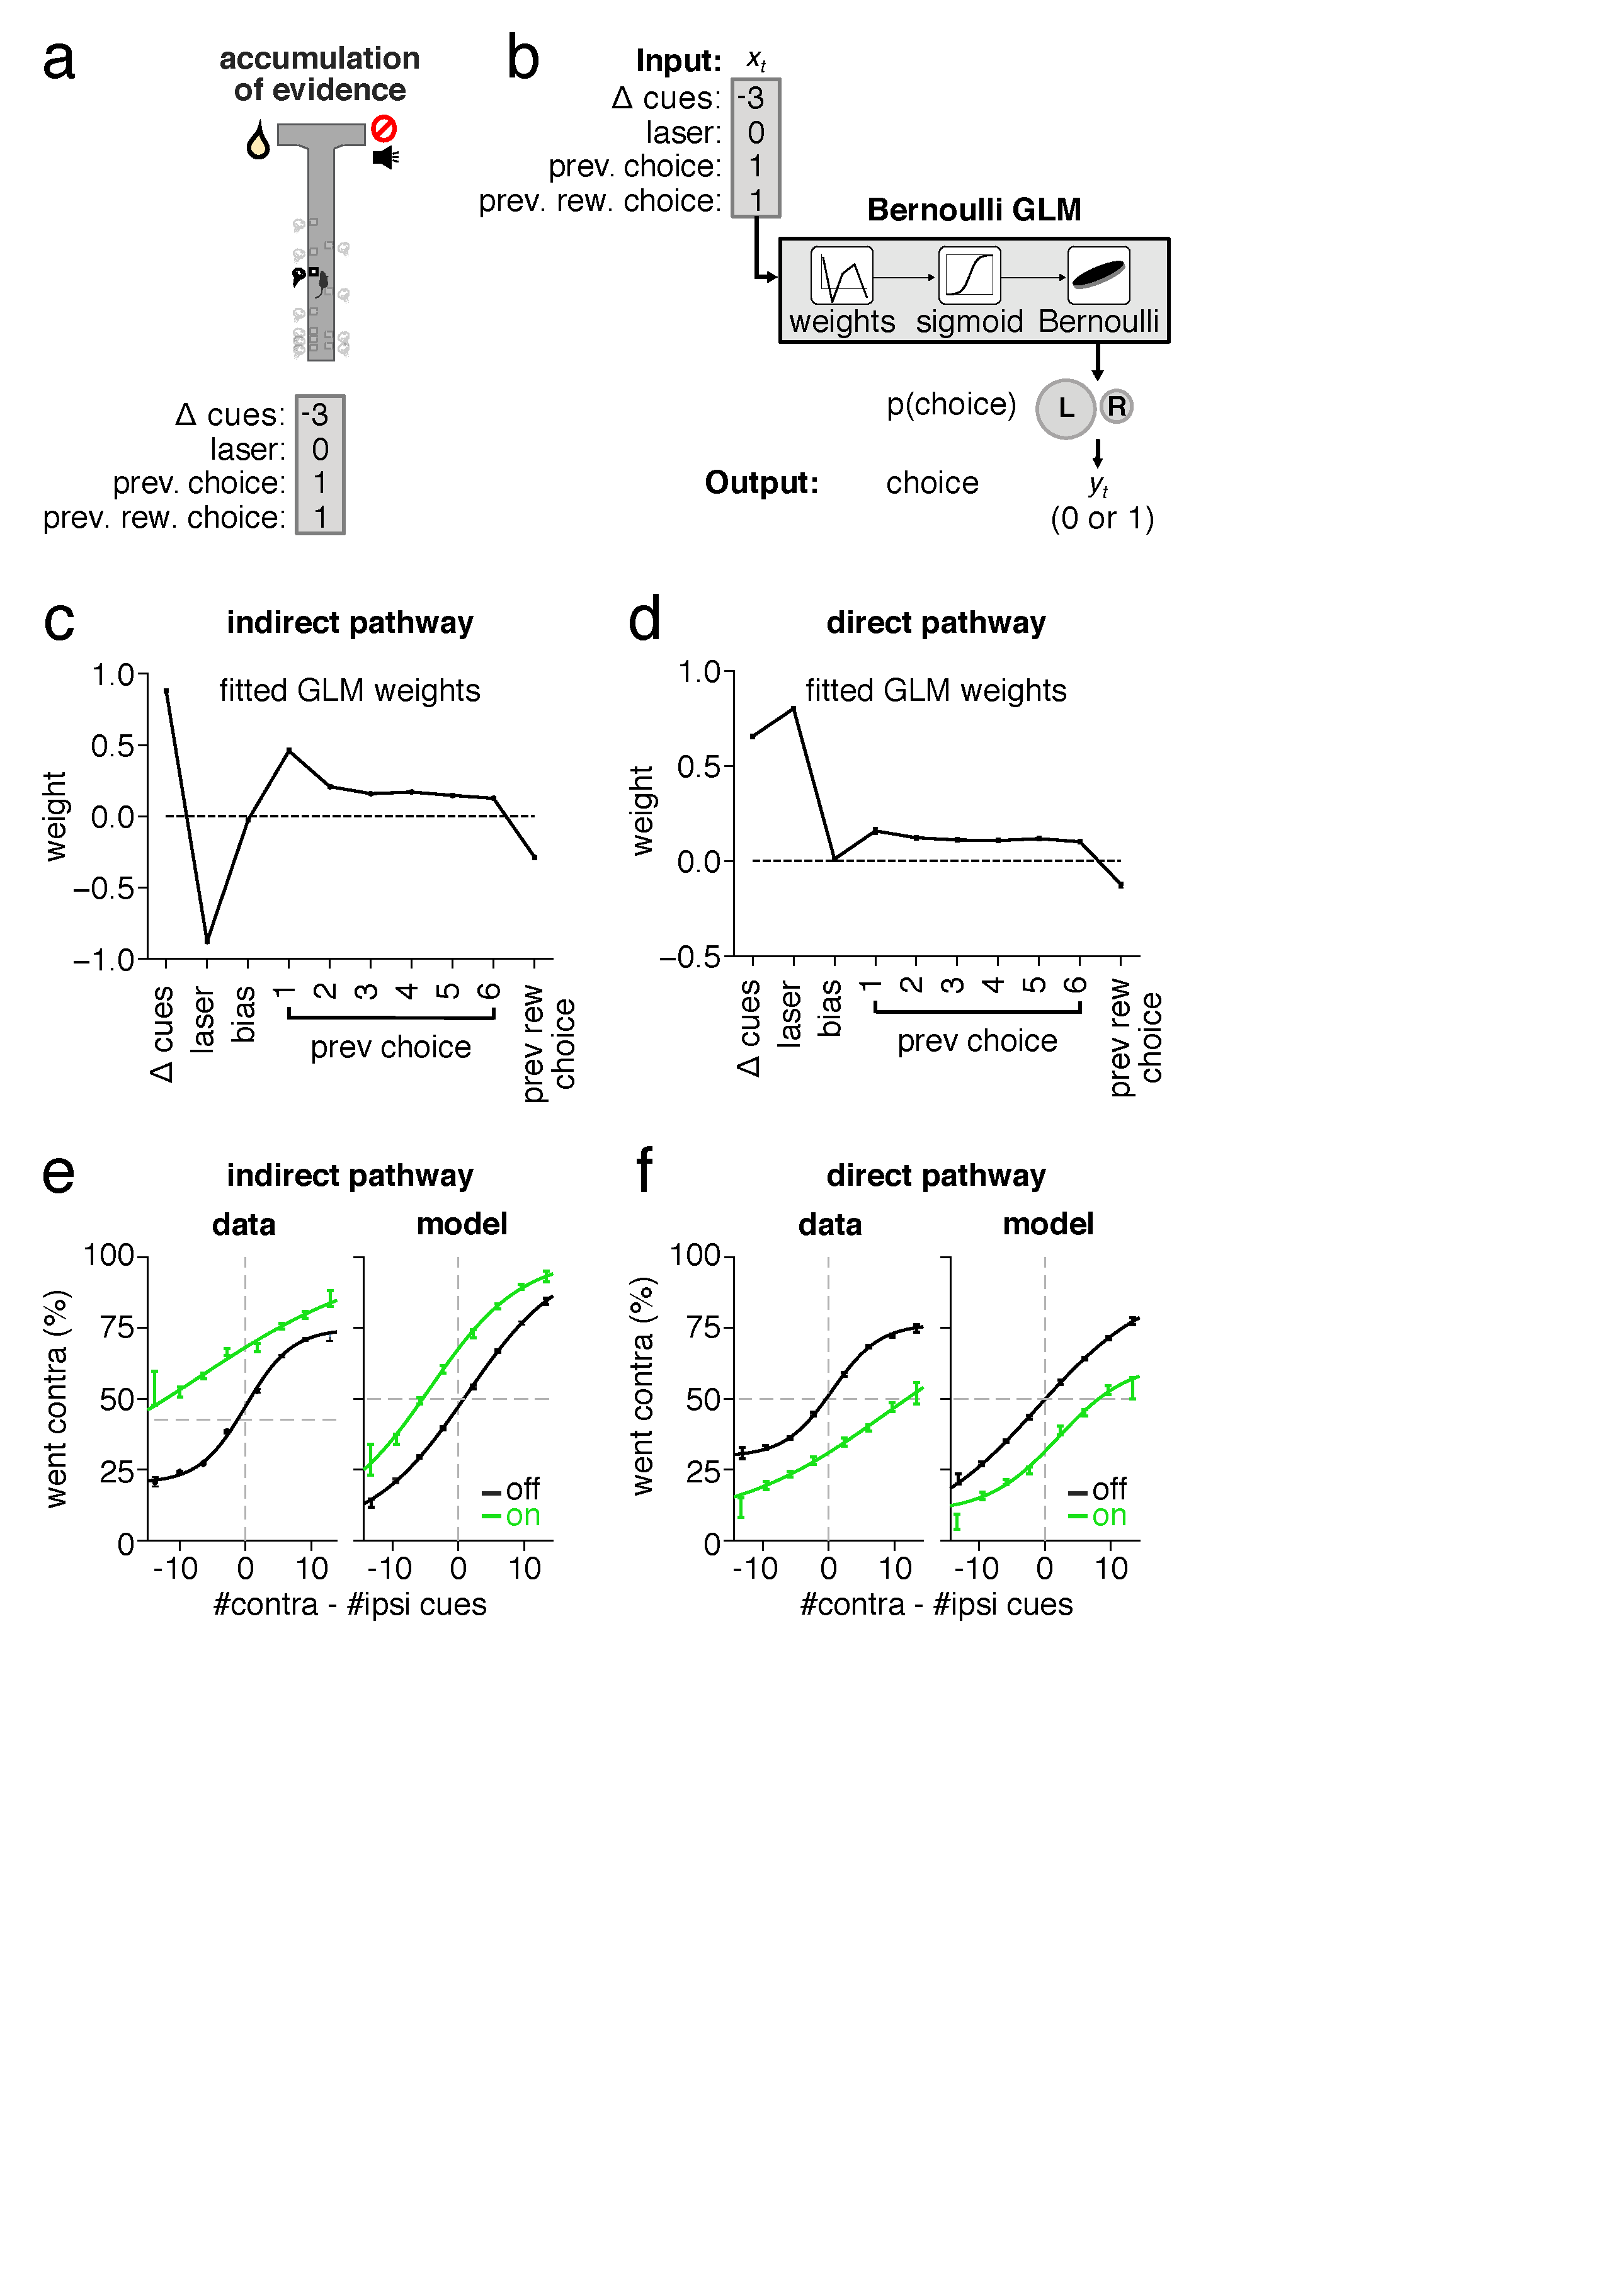
\includegraphics[width=0.70\linewidth]{ch2-glmhmm/glmhmm-figures/Fig4.pdf}
    \caption[A GLM reveals that sensory evidence, dorsomedial striatum pathway inhibition and trial history predict choice during the evidence accumulation task, but does not precisely recapitulate the shape of the psychometric curve.]{\textbf{A GLM reveals that sensory evidence, dorsomedial striatum pathway inhibition and trial history predict choice during the evidence accumulation task, but does not precisely recapitulate the shape of the psychometric curve.} (a) Schematic of the evidence accumulation task and the coding of the external covariates for an example trial.  (b) Schematic of the Bernoulli GLM for an example trial, showing the relationship between external covariates (inputs) and choice on each trial. On each trial, a set of GLM weights maps each input ($\Delta$ cues, laser, bias, previous choice, and existence of a previous rewarded choice) to the probability of each outcome through a sigmoid function, which gives the probability of a “righward” choice on the current trial. (c) Fitted GLM weights using aggregated data from all mice in the indirect pathway DMS inhibition group. The magnitude of each weight indicates the relative importance of that covariate in predicting choice, whereas the sign of the weight indicates the direction of the effect (e.g. a negative laser weight indicates that if inhibition is in the right hemisphere, the mice will be more likely to turn left, while a positive weight on previous choice indicates that if the previous choice was to the right, in the current trial this will bias the mice to turn right again). }
    \label{fig:glmhmm:4}
  \end{center}
  \vspace{-1.5cm}
\end{figure}
\begin{figure}[t!]
  \contcaption{Error bars denote ($\pm$1) posterior standard deviation credible intervals. (d) Same as c but for mice receiving DMS direct pathway inhibition. (e) Fraction of contralateral choice trials as a function of the difference in contralateral versus ipsilateral cues  for laser off (black) and on (green) trials, for mice receiving indirect pathway DMS inhibition for the data (left) and for simulations of the model (right). Error bars denote 95\% confidence intervals around the fraction of choices in each bin of the data; solid curves denote logistic fits (n=13 mice, n = 46,313 laser off and n = 8,570 laser on trials).  (f) Same as e but for the mice receiving direct pathway inhibition of the DMS (n=13 mice, n = 41,250 laser off and n = 7,927 laser on trials).}% Continued caption
\end{figure}

We fit the GLM to aggregated behavioral data from mice inhibited in each DMS pathway and found that sensory evidence, trial history and optical inhibition all contributed to predicting choice (Fig. \ref{fig:glmhmm:4}c,d). As expected, the effect of inhibition of each pathway was large and opposite in sign. However, the GLM did not accurately capture the animals’ psychometric curve, describing the probability of a rightward choice as a function of the sensory evidence (Fig. \ref{fig:glmhmm:4}e,f). This led us to consider variants of the standard GLM that might better account for choice behavior.